\documentclass[10pt, a4paper]{article}
\usepackage[latin1]{inputenc}
\usepackage{amsmath}
\usepackage{amsfonts}
\usepackage{amssymb}
\usepackage{graphicx}
\usepackage{xcolor}
\usepackage{float}
\usepackage{hyperref}
\usepackage{booktabs}
\usepackage[normalem]{ulem}
\usepackage{cite}



% Forcequit autonumbering
\pagenumbering{gobble}


%% Multicolumns
\usepackage{multicol}
\setlength{\columnsep}{1cm}


% Margin to left and middle
\usepackage[margin={2cm,1cm}]{geometry}


\title{Imaterialist challenge - Report}
\author{Mick van Hulst \and Dennis Verheijden \and Roel van der burg \and Brian Westerweel \and Joost Besseling}

\begin{document}
    \maketitle
    \section{Exploratory Data Analysis}
    The dataset that the challenge provides consists of a training, test and validation set, which in turn consist of: 
    \begin{itemize}
        \item 1.014.544 training images;
        \item 228 labels in the training dataset;
        \item 39.706 test images;
        \item 9.897 validation images;
        \item 225 labels in validation set.
    \end{itemize}
    We're interested in the distributions of the data such that we can prepare our models accordingly. Figure \ref{fig:data_dist_train} and \ref{fig:data_dist_val} visualise the distribution of the labels for the training and validation dataset respectively. We observe that the labels aren't evenly distributed, but the distribution between the training and validation dataset seems comparable.
	\begin{figure}[H]
        \centering
        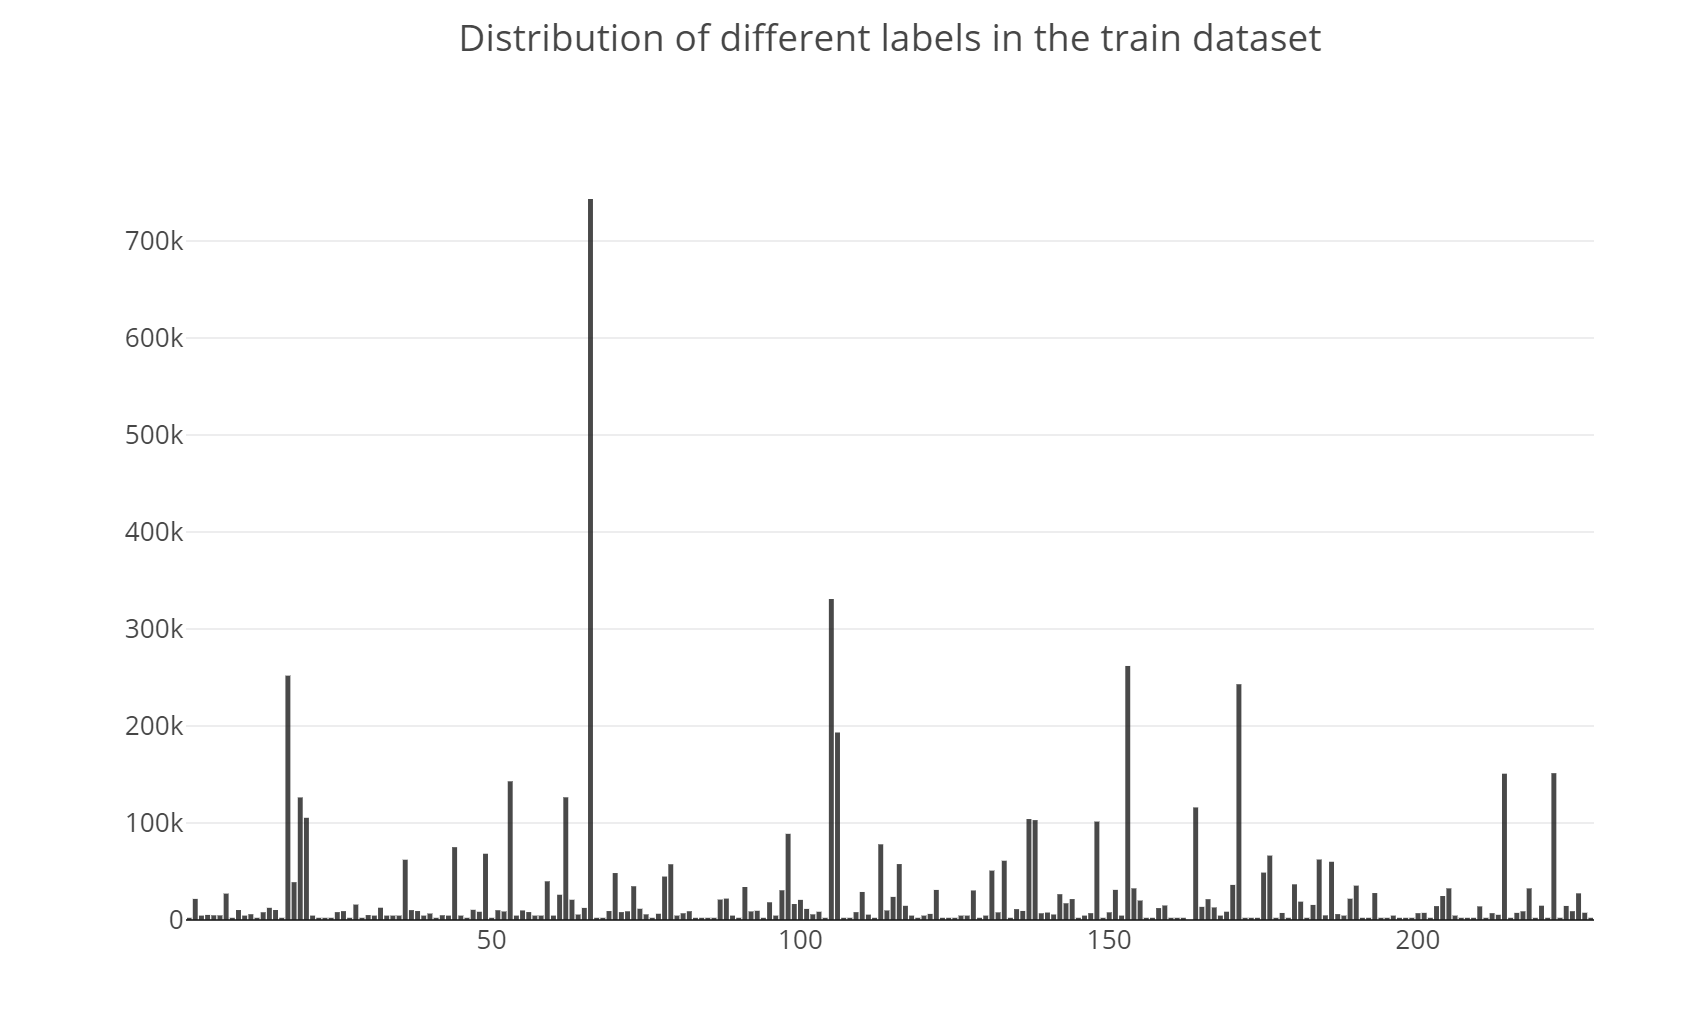
\includegraphics[scale=.4]{img_imaterialist/dist_labels_train.png}
        \caption{Data distribution training set}
        \label{fig:data_dist_train}
    \end{figure}

	\begin{figure}[H]
        \centering
        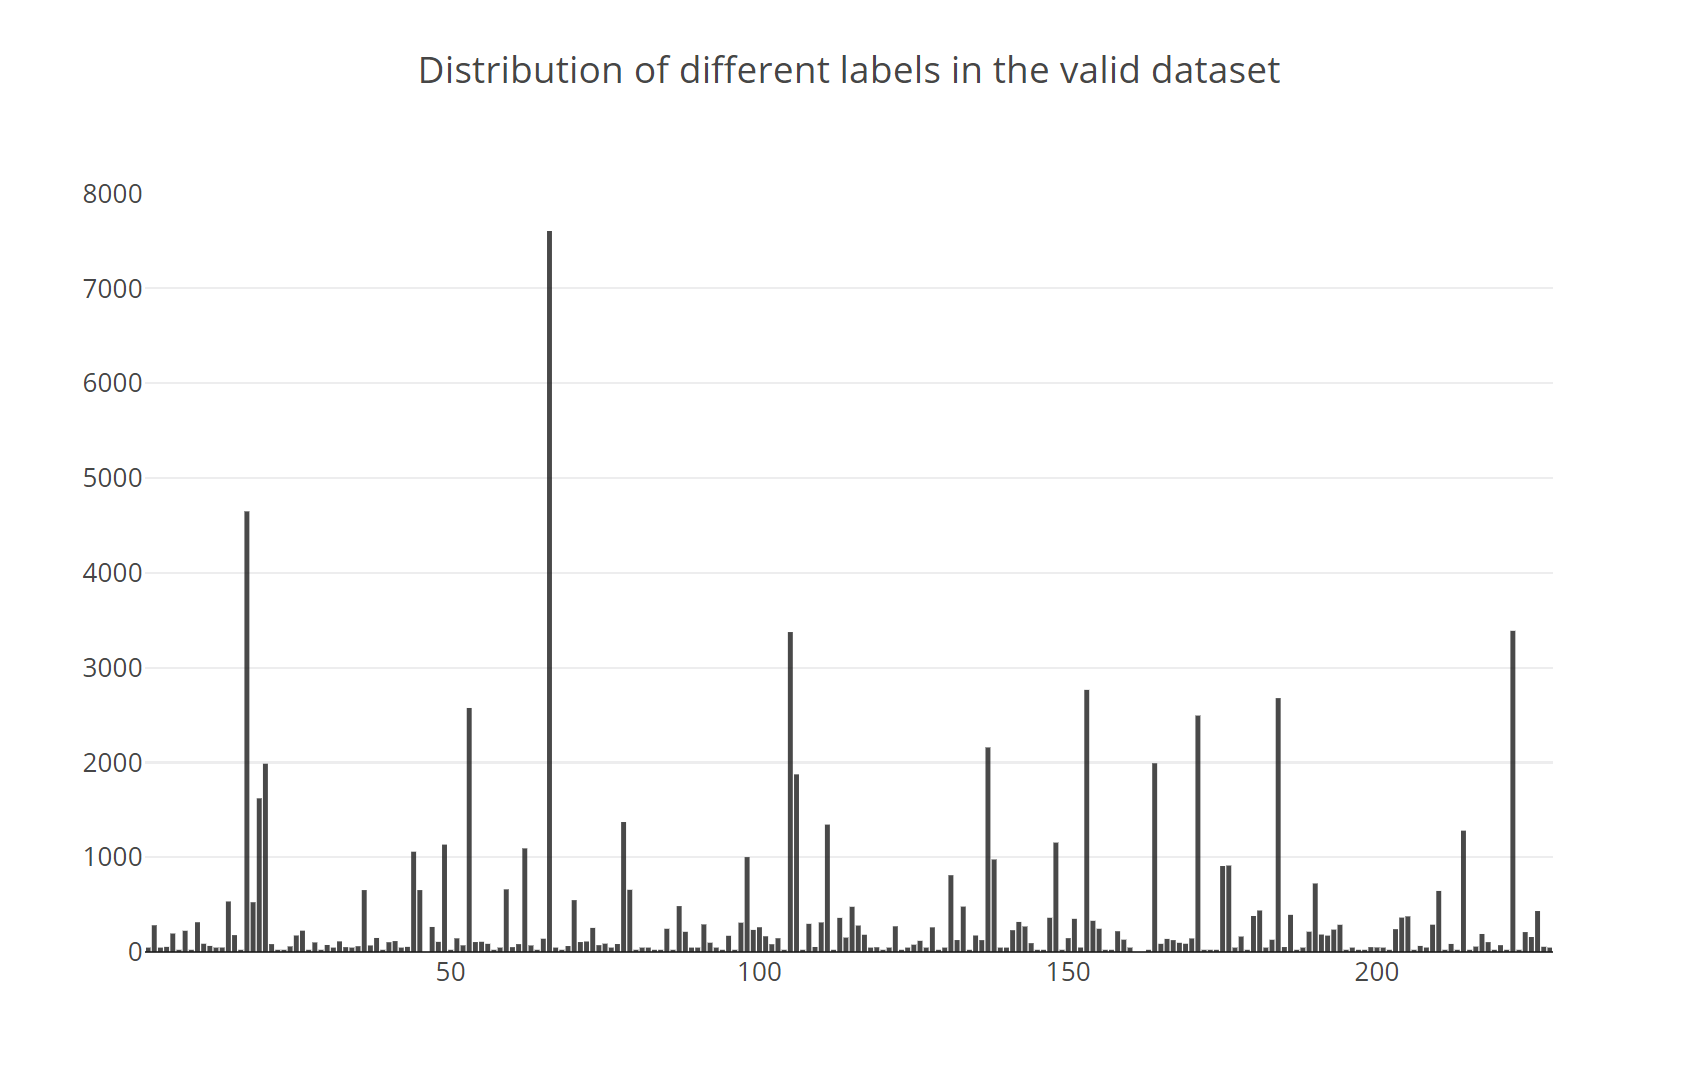
\includegraphics[scale=.4]{img_imaterialist/dist_labels_validation.png}
        \caption{Data distribution validation set}
        \label{fig:data_dist_val}
    \end{figure}
    To get a feeling for the dataset we also visualise some images and observe that for some labels there are no clear characteristics that define the corresponding label (see Figure \ref{fig:img_example}). From this observation we conclude that it would be hard for a human to differentiate between the labels without knowing what the labels mean exactly. We believe that there's some structure to the labels, meaning that there might be some tree-like structure that explains the different combinations between the labels, however, this is not something that the challenge provides so we cannot use this to e.g. define weights when classifying. This is something we'll have to define ourselves.
	\begin{figure}[H]
        \centering
        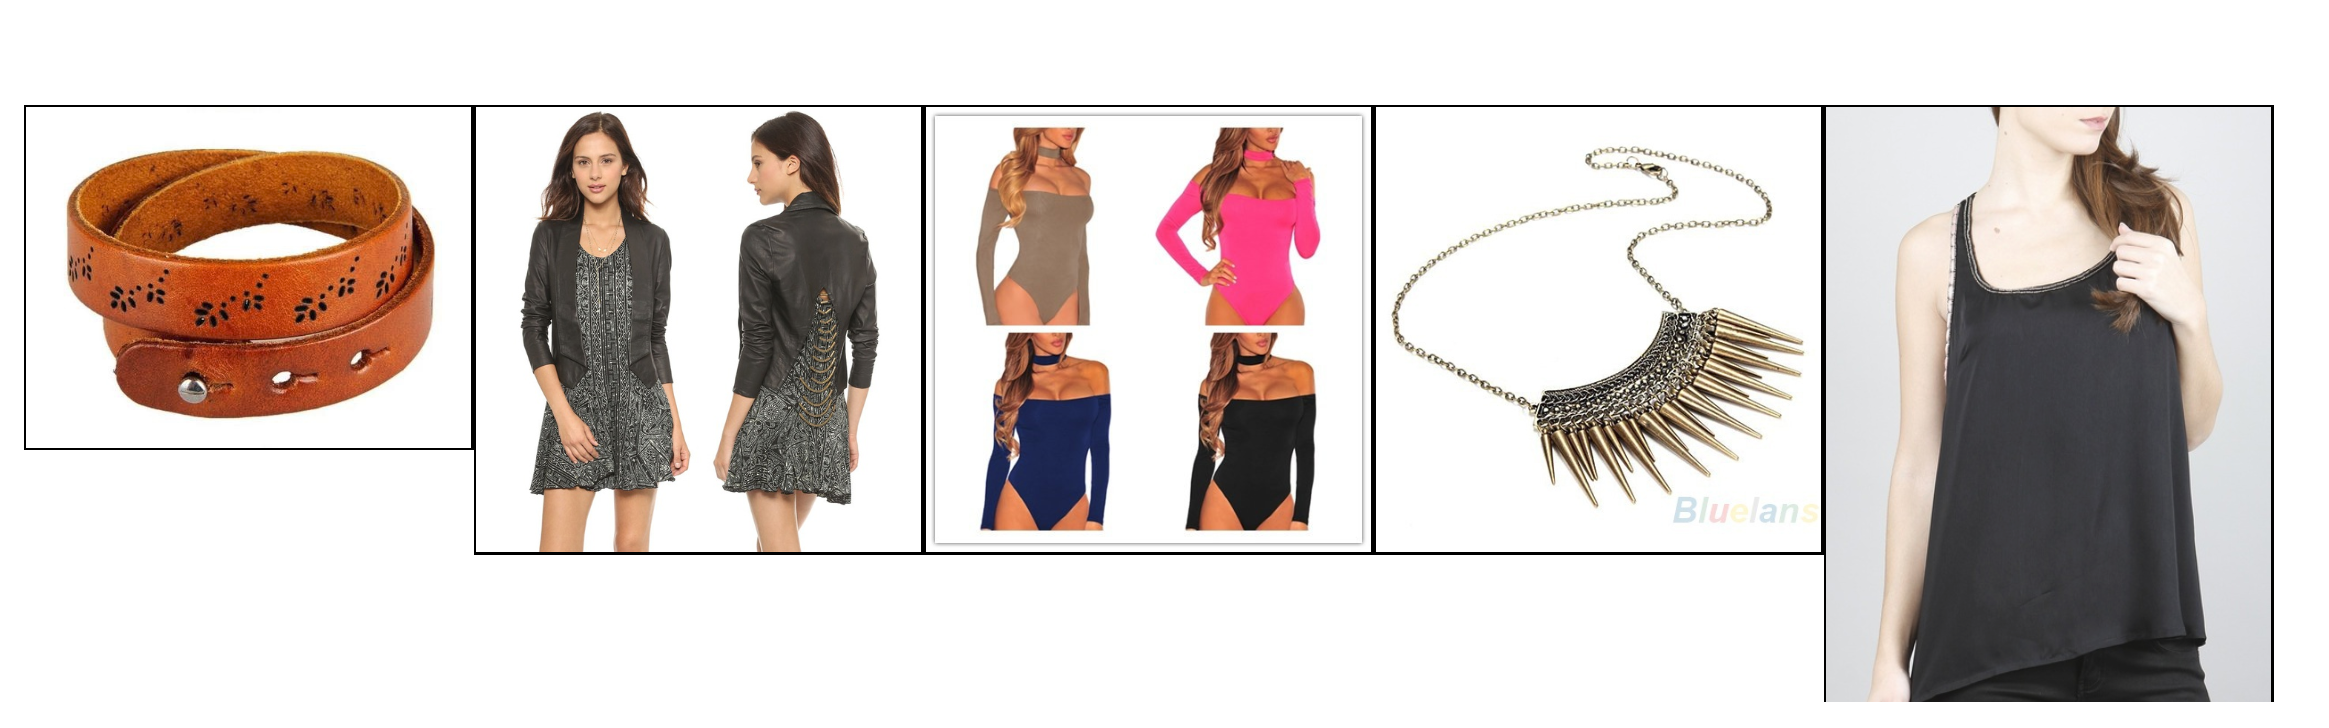
\includegraphics[scale=.4]{img_imaterialist/label_24.jpg}
        \caption{Example image label 24}
        \label{fig:img_example}
    \end{figure}
    
    Source: \url{https://www.kaggle.com/shivamb/imaterialist-fashion-eda-object-detection-colors}
    



\end{document}